\documentclass{article}
\usepackage[T1]{fontenc}
\usepackage[utf8]{inputenc}
\usepackage[margin=2cm]{geometry}
\usepackage{graphicx}
\usepackage{parskip}

\title{Zadanie 3 - Raport}
\author{Jan Stusio}
\date{Kwiecień 2024}

\begin{document}

\maketitle

\section{Wstęp}

Celem zadania jest zaimplementowanie algorytmu MinMax i alpha pruning dla gry w kółko i krzyżyk.


\section{Implementacja}

Przygotowałem konsolową grę w kółko i krzyżyk. Gracz wykonuje tylko decyzje Mina, a komputer ruchy Maxa. Przed każdym ruchem (poza początkowym) w konsoli wyświetlają się zewaulowane akcje przez algorytm MinMax bez oraz z alpha pruningiem.

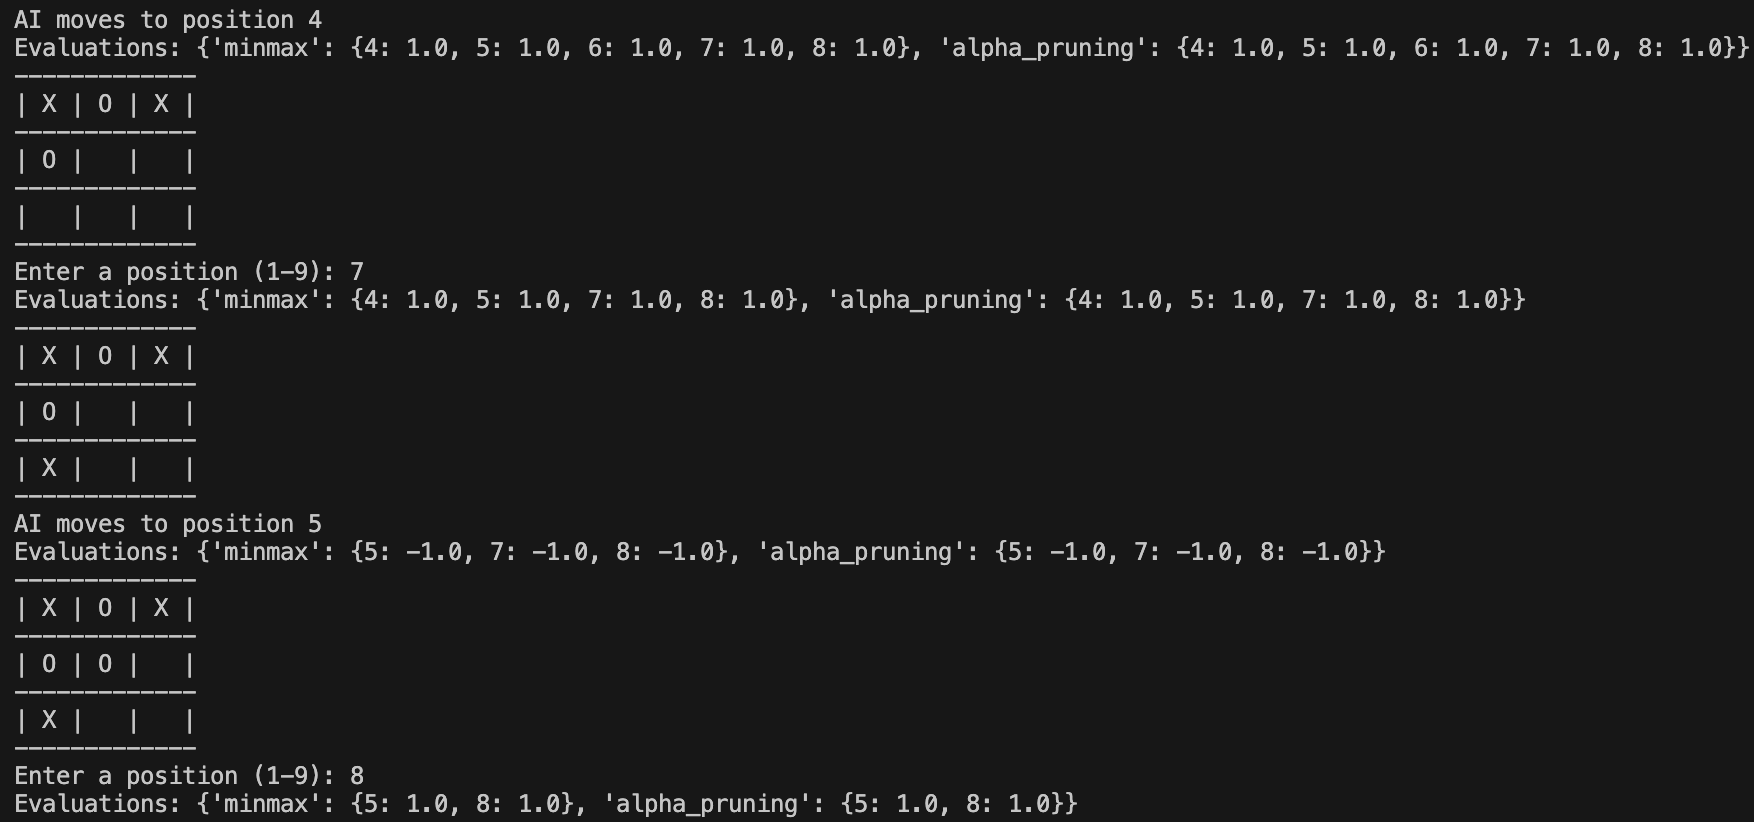
\includegraphics[width=18cm, height=8cm]{Screenshot 2024-04-07 at 22.18.07.png}

Algorytm MinMax zaimplementowałem w klasie o tej samej nazwie zgodnie z sygnaturami sugerowanymi w treści zadania zgodnie z rekurencyjnym pseudokodem podanym na wykładach. Nie implementowałem heurystyki.


Gra zaimplementowana jest w klasie TikTakToe.

\section{Badania}

Badałem:

\quad 1. Liczbę odwiedzonych węzłów oraz głębokość drzewa dla wszystkich możliwych początkowych stanów gry (9 opcji) oraz 3 wybranych stanów „ze środka” gry

\quad 2. Jak alpha pruning wpływa na głębokość drzewa i liczbę odwiedzanych węzłów

\quad 3. Zależności czasu wykonania algorytmu dla pojedynczego ruchu w zależności od postępu w grze z i bez alpha pruningu

\section{Wyniki badań}

\subsection{Odwiedzanie węzłów i głębokość drzewa}

Badane stany "środka" gry:\\

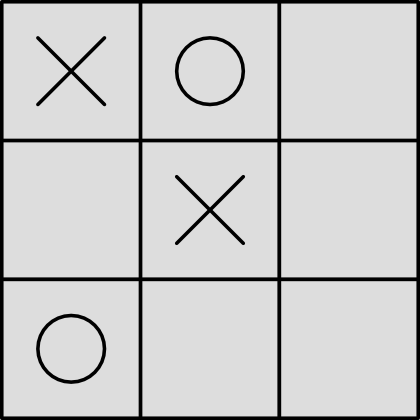
\includegraphics[width=5cm, height=5cm]{midgamestate1.png}
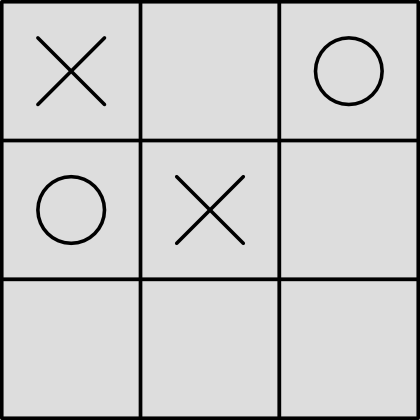
\includegraphics[width=5cm, height=5cm]{midgamestate2.png}
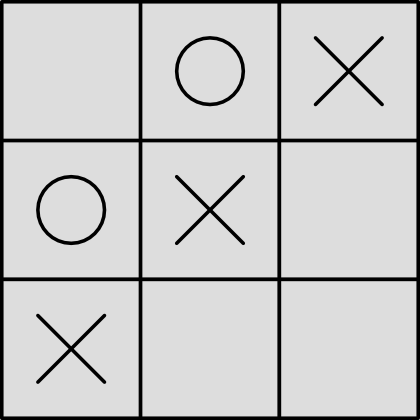
\includegraphics[width=5cm, height=5cm]{midgamestate3.png}

\begin{minipage}[t]{0.6667\textwidth}

\smallskip
\textbf{MinMax:}\\
Initial state 1, Visited nodes: 59705\\\\
Initial state 2, Visited nodes: 63905\\\\
Initial state 3, Visited nodes: 59705\\\\
Initial state 4, Visited nodes: 63905\\\\
Initial state 5, Visited nodes: 55505\\\\
Initial state 6, Visited nodes: 63905\\\\
Initial state 7, Visited nodes: 59705\\\\
Initial state 8, Visited nodes: 63905\\\\
Initial state 9, Visited nodes: 59705\\\\
Mid-game state 1, Visited nodes: 210\\\\
Mid-game state 2, Visited nodes: 1\\\\
Mid-game state 3, Visited nodes: 1\\\\
\textbf{Average leaf depth in all cases: 9}\\
\end{minipage}
\begin{minipage}[t]{1.3333\textwidth}
\smallskip
\textbf{Alpha pruning:}\\
Initial state 1, Visited nodes: 61110\\
Average leaf depth: 6.73630831643002\\
Initial state 2, Visited nodes: 65930\\
Average leaf depth: 6.811814345991561\\
Initial state 3, Visited nodes: 61068\\
Average leaf depth: 6.835830212234707\\
Initial state 4, Visited nodes: 67122\\
Average leaf depth: 6.837768866204885\\
Initial state 5, Visited nodes: 57466\\
Average leaf depth: 6.826036866359447\\
Initial state 6, Visited nodes: 66480\\
Average leaf depth: 6.838386140870755\\
Initial state 7, Visited nodes: 61073\\
Average leaf depth: 6.809209167871154\\
Initial state 8, Visited nodes: 66081\\
Average leaf depth: 6.812868632707775\\
Initial state 9, Visited nodes: 61311\\
Average leaf depth: 6.800195090229231\\
Mid-game state 1, Visited nodes: 171\\
Average leaf depth: 6.803769937167714\\
Mid-game state 2, Visited nodes: 1\\
Average leaf depth: 6.803479381443299\\
Mid-game state 3, Visited nodes: 1\\
Average leaf depth: 6.803511032372363\\
\textbf{Average leaf depth in all cases: $\sim$6.8}\\

\end{minipage}

\subsection{Pomiar czasu}

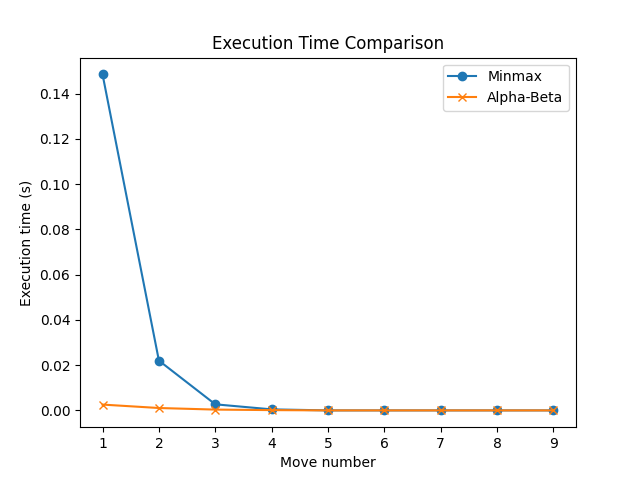
\includegraphics[width=7.7cm, height=6cm]{execution_time_comparison2.png}


\section{Wnioski}

Czas wykonania algorytmu dla pojedynczego ruchu w zależności od postępu w grze bez alpha pruningu spada w miarę postępu gry, co jest zgodne z oczekiwaniami.
Dla alpha pruningu czas wykonania jest znacznie krótszy w początkowych stanach gry. W miarę postępu gry różnica w czasie wykonania dla obu algorytmów maleje, co jest zgodne z oczekiwaniami.
Głębokość drzewa dla alpha pruningu jest znacznie mniejsza niż dla MinMaxa bez niego, ale liczba odwiedzonych węzłów jest nieznacznie większa.

\end{document}
